\documentclass{article}

\usepackage{fullpage}
\usepackage{color}
\usepackage{amsmath}
\usepackage{url}
\usepackage{verbatim}
\usepackage{graphicx}
\usepackage{parskip}
\usepackage{amssymb}
\usepackage{nicefrac}
\usepackage{listings}


% Colors
\definecolor{blu}{rgb}{0,0,1}
\def\blu#1{{\color{blu}#1}}
\definecolor{gre}{rgb}{0,.5,0}
\def\gre#1{{\color{gre}#1}}
\definecolor{red}{rgb}{1,0,0}
\def\red#1{{\color{red}#1}}
\def\norm#1{\|#1\|}

% Math
\def\R{\mathbb{R}}
\def\argmax{\mathop{\rm arg\,max}}
\def\argmin{\mathop{\rm arg\,min}}
\newcommand{\mat}[1]{\begin{bmatrix}#1\end{bmatrix}}
\newcommand{\alignStar}[1]{\begin{align*}#1\end{align*}}
\def\half{\frac 1 2}

% LaTeX
\newcommand{\fig}[2]{\includegraphics[width=#1\textwidth]{#2}}
\newcommand{\centerfig}[2]{\begin{center}\includegraphics[width=#1\textwidth]{#2}\end{center}}
\newcommand{\matCode}[1]{\lstinputlisting[language=Matlab]{a2f/#1.m}}
\def\items#1{\begin{itemize}#1\end{itemize}}
\def\enum#1{\begin{enumerate}#1\end{enumerate}}

\def\rubric#1{\gre{Rubric: \{#1\}}}{}
\graphicspath{ {..figs/} }

\begin{document}

\title{CPSC 340 Assignment 2 Report}
\author{}
\date{}
\maketitle
\vspace{-4em}

\section{Naive Bayes}

\subsection{Naive Bayes by Hand}

\blu{(a) Compute the estimates of the class prior probabilities} (you don't need to show any work):
\items{
\item $p(y = 1) = 0.6$.
\item $p(y = 0) = 0.4$. 
}

\blu{(b) Compute the estimates of the 4 conditional probabilities required by naive Bayes for this example}  (you don't need to show any work):
\items{
\item $p(x_1 = 1 | y = 1) = 0.5$.
\item $p(x_2 = 0 | y = 1) = 0.33$.
\item $p(x_1 = 1 | y = 0) = 1$.
\item $p(x_2 = 0 | y = 0) = 0.75$.
}

\blu{(c) Under the naive Bayes model and your estimates of the above probabilities, what is the most likely label for the test example? (Show your work.)}

$$p(y = 1 | x_1 = 1, x_2 = 0) = p(x_1 = 1 | y = 1) * p(x_2 = 0 | y = 1) * p(y = 1)$$
$$= 0.5 * 0.33 * 0.6$$
$$= 0.1$$

$$p(y = 0 | x_1 = 1, x_2 = 0) = p(x_1 = 1 | y = 0) * p(x_2 = 0 | y = 0) * p(y = 0)$$
$$= 1 * 0.75 * 0.4$$
$$= 0.3$$

As $0.3 > 0.1$, the most likely label for the test example is $0$.


\subsection{Bag of Words}

\blu{Answer the following}:
\enum{
\item Which word corresponds to column 50 of $X$? lunar
\item Which words are present in training example 500? car, fact, gun, video
\item Which newsgroup name does training example 500 come from? talk.*
}

\subsection{Naive Bayes Implementation}

\blu{Modify this function so that \texttt{p\_xy} correctly
computes the conditional probabilities of these values based on the
frequencies in the data set. Hand in your code and the validation error that you obtain.
Also, briefly comment on the accuracy as compared to the random forest and scikit-learn's naive Bayes implementation.}

The code can be found at $code/naive\_bayes.py$.

The random forest: 0.203\\
The validation error obtained (before implementing Laplace smoothing): 0.188\\
The sklearn validation error: 0.187

Our validation error is quite close to the sklearn validation error, meaning our implementation was mostly correct.

\subsection{Laplace smoothing}

\blu{Do the following}:
\enum{
\item Modify your code so that it uses Laplace smoothing, with $\beta$ as a parameter taken in by the constructor. \\\\Done, the code can be found at $code/naive\_bayes.py$.
\item Did you need to modify your fit function, predict function, or both? \\\\Only the fit function needed to be modified.
\item Take a look at the documentation for the scikit-learn version of naive Bayes the code is using. How much Laplace smoothing does it use by default? Using the same amount of smoothing with your code, do you get the same results? \\\\It uses 1 as the default value for Laplace smoothing. \\\\The validation error obtained (after using a value of 1 for Laplace smoothing): 0.187. We do indeed get the same amount of smoothing.
}
	

\subsection{Runtime of Naive Bayes for Discrete Data}

\blu{What is the cost of classifying $t$ test examples with the model?}

The cost of classifying $t$ examples would be $O(tkd)$.

\textit{Assume finding the probability of $k$ is $O(1)$ as it should be found in the training phase.}

\textit{Assume finding the conditional probability of $d = c$ is $O(1)$ as it should be found in the training phase, and stored in a array where the value is accessible with $d$, $k$ and $c$.}

\textbf{The explanation is as follows:}

For each testing object, we must find the greatest conditional probability of each $k$ given all $d$ features, where some $d_n$ equals some $c$, so we may classify it as that k. In order to do that, we first find the probability of $k$. 

Then, for each feature, we find the conditional probability of $d = c$ given $k$, and multiply it by our probability of $k$.  This gives us the conditional probability of our current $k$ given all $d$ features. If it is greater than the current greatest conditional probability, we replace it and its label.

Finally, we can classify the testing object as the label that has the current greatest conditional probability.

Looping through all the features and finding the conditional probability for them to multiply all together is $O(d)$.
This is done for each $k$, which is $O(kd)$, to find what we should label $t$.
Finally, this is done for each $t$, which is $O(tkd)$, as we must label every $t$.



\section{Random Forests}

\subsection{Implementation}


\blu{
\enum{
\item Why doesn't the random tree model have a training error of 0?
\item Create a class \texttt{RandomForest} in a file called \texttt{random\string_forest.py} that takes in hyperparameters \texttt{num\string_trees} and \texttt{max\string_depth} and
fits \texttt{num\string_trees} random trees each with maximum depth \texttt{max\string_depth}. For prediction, have all trees predict and then take the mode.
\item Using 50 trees, and a max depth of $\infty$, report the training and testing error. Compare this to what we got with a single \texttt{DecisionTree} and with a single \texttt{RandomTree}. Are the results what you expected? Discuss.
\item Compare your implementation with scikit-learn's \texttt{RandomForestClassifier} for both speed and accuracy, and briefly discuss. You can use all default hyperparameters if you wish, or you can try changing them.
}
}

\subsection{Very-Short Answer Questions}
\rubric{reasoning:3}

\blu{\enum{
\item What is a a disadvantage of using a very-large number of trees in a random forest classifier?
\item Your random forest classifier has a training error of 0 and a very high test error. Which ones of the following could help performance?
\enum{
\item Increase the maximum depth of the trees in your forest.
\item Decrease the maximum depth of the trees in your forest.
\item Increase the amout of data you consider for each tree (Collect more data and use $2n$ objects instead of $n$).
\item Decrease the amount of data you consider for each tree (Use $0.8n$ objects instead of $n$).
\item Increase the number of features you consider for each tree.
\item Decrease the number of features you consider for each tree.
}
\item Suppose that you were training on raw audio segments and trying to recognize vowel sounds. What could you do to encourage the final classifier to be invariant to translation?
}
}

\section{Clustering}

\subsection{Selecting among $k$-means Initializations}

 {\enum{
 \blu{\item In the \emph{kmeans.py} file, add a new function called \emph{error} that takes the same input as the \emph{predict} function but that returns the value of this above objective function. Hand in your code.} \\\\ Done, the code can be found in $code/kmeans.py$.
 \blu{\item What trend do you observe if you print the value of \emph{error} after each iteration of the $k$-means algorithm?} \\\\ Our error gets less and less with each iteration of the algorithm. The difference between iterations gets smaller and smaller, approaching the error found when no clusters change.
 \blu{\item Using \texttt{plot\_2dclustering}, output the clustering obtained by running $k$-means 50 times (with $k=4$) and taking the one with the lowest error.} \\\\ 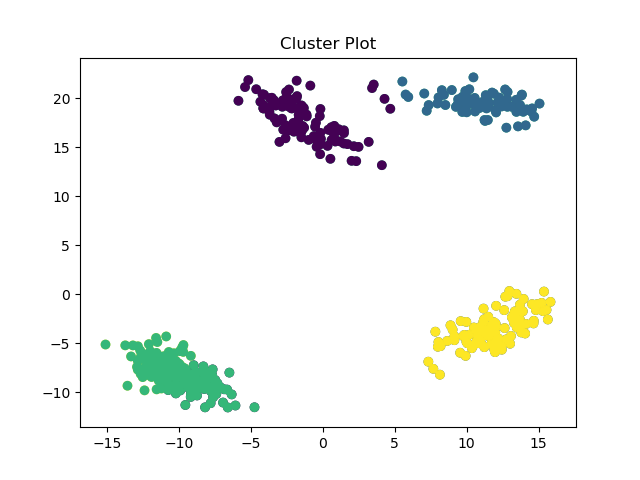
\includegraphics{../figs/kmeans_3_1}
 \blu{\item Looking at the hyperparameters of scikit-learn's \texttt{KMeans}, explain the first four (\texttt{n\_clusters}, \texttt{init}, \texttt{n\_init}, \texttt{max\_iter}) very briefly.} \\\\ n\_clusters indicates the number of clusters that we want to classify in the end. \\init specifies how we want to choose our centroids. \\n\_init specifies the number of times we want to initialize. \\max\_iter specifies the max number of times we can iterate the k\_mean algorithm for.
 }}


\subsection{Selecting $k$ in $k$-means}

 \enum{
 \blu{\item Explain why the \emph{error} function should not be used to choose $k$.} \\\\ It doesn't make sense to use error to pick k, because our most optimal value would be k = n, because then each point would be its own cluster, giving us an error of 0. But then at that point we wouldn't even be clustering.
 \blu{\item Explain why even evaluating the \emph{error} function on test data still wouldn't be a suitable approach to choosing $k$.} \\\\\ Same thing as above. Even if we use different data, we would still get the smallest error if we set k = n. Again, we wouldn't even be clustering.
 \blu{\item Hand in a plot of the minimum error found across 50 random initializations, as a function of $k$, taking $k$ from $1$ to $10$.} \\\\ 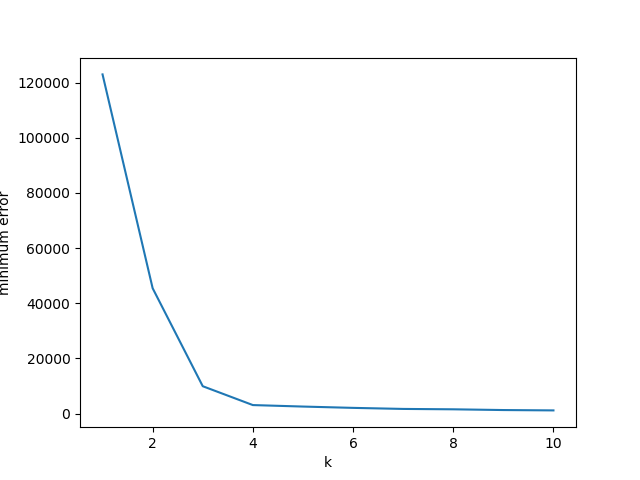
\includegraphics{../figs/kmeans_3_2}
 \blu{\item The \emph{elbow method} for choosing $k$ consists of looking at the above plot and visually trying to choose the $k$ that makes the sharpest ``elbow" (the biggest change in slope). What values of $k$ might be reasonable according to this method? Note: there is not a single correct answer here; it is somewhat open to interpretation and there is a range of reasonable answers.} \\\\ Reasonable values would include 2, 3 or 4, although 2 and 3 makes the most noticeable difference in slope.
}

\subsection{$k$-medians}

 \enum{
 \blu{\item Using the \texttt{plot\_2dclustering} function, output the clustering obtained by running $k$-means 50 times (with $k=4$)  and taking the one with the lowest error. Are you satisfied with the result?}\\\\ It seems to have done a fine job classifying the clusters. However, the error appears to be extremely high.
 \blu{\item What values of $k$ might be chosen by the elbow method for this dataset?} \\\\ You would pick 2 or 3 as they appear to give the sharpest slope. 4 doesn't seem to give much of a slope.
 \blu{\item Implement the $k$-\emph{medians} algorithm, which assigns examples to the nearest $w_c$ in the L1-norm and to updates the $w_c$ by setting them to the ``median" of the points assigned to the cluster (we define the $d$-dimensional median as the concatenation of the median of the points along each dimension). Hand in your code and plot obtained with 50 random initializations for $k = 4$.} \\\\ 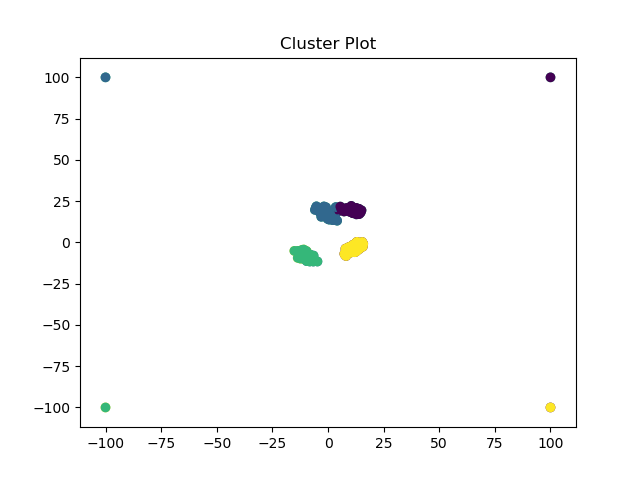
\includegraphics{../figs/kmeans_3_3}
\blu{\item Using the L1-norm version of the error (where $y_i$ now represents the closest median in the L1-norm),
what value of $k$ would be chosen by the elbow method under this strategy? Are you satisfied with this result?} \\\\ Again, 2, 3 or 4 would be reasonable values to pick. We might tend towards 4 as the graph provided by kmeans has less of a slope tending towards 4 and we can appear to identify 4 "individual" clusters in the plot.
}

\subsection{Density-Based Clustering}

\enum{
\blu{\item The 4 ``true" clusters.} \\\\ eps = 3, min\_samples = 3
\blu{\item 3 clusters (merging the top two, which also seems like a reasonable interpretaition).} \\\\ eps = 6, min\_samples = 6
\blu{\item 2 clusters.} \\\\ eps = 15, min\_samples = 2
\blu{\item 1 cluster (consisting of the non-outlier points).} \\\\ eps = 30, min\_samples = 2
}



\subsection{Very-Short Answer Questions}

\enum{
\blu{\item Does the standard $k$-means clustering algorithm always yield the optimal clustering solution for a given $k$?}\\\\ No, it doesn't. At times, we can get weird initializations, which will lead the means to sometimes converge to weird locations and classify weirdly. For example, if there are two clusters that are somewhat together, in some initializations, we might correctly label the two as individual clusters, in other initializations, there might be a mean smack dab in the two, causing it to be labelled as one big cluster.
\blu{\item If your set out to minimize the distance between each point and its mean in a $k$-means clustering, what value of $k$ minimizes this cost? Is this value useful?} \\\\ k = n, where n is equal to the number of points. This value isn't useful at all, as we are no longer identifying clusters, but rather each individual point.
\blu{\item Describe a dataset with $k$ clusters where $k$-means would not be able to find the true clusters.} \\\\ Imagine that we have two clusters. One that looks like a horseshoe, and the other that looks like an upside down horseshoe. They would then be positioned such that the two would almost be "linking" together. Here, k-means would not be able identify that there are two clusters. If we set k = 2, the model would guess that the "intersection" point between the two horseshoes is a cluster in itself. K-means is not able to accurately identify a pattern like this where the real cluster appears like a horseshoe - rather, it can only identify circular, blob-like clusters.
\blu{\item Suppose that you had only two features and that they have very-different scales (like kilograms vs. milligrams). How would this affect the result of density-based clustering?} \\\\ As k-means simply clusters points based on their difference in distance - each features "idea" of distance should be similar, otherwise you are going to get very skewed results that are not based on the actual distance of the points. For example, a scale of miligrams might treat a difference of 1 gram as huge - whereas a scale of kilograms might treat a difference of 1 gram as very small. Hence, you might get clusters that are entirely dependent on the scale treating the difference as very small, or clusters that are not represented due to the scale treating the difference as very big.
\blu{\item Name a key advantage and drawback of using a supervised outlier detection method rather than an unsupervised method?} \\\\ A disadvantage: experience overfitting on the training dataset - only know how to identify outliers for a specific training dataset (the point you've seen) - can't really detect any outliers on any new data. \\\\ An advantage: unsupervised learning can only detect outliers through a difference of "distance" in the features - it isn't actually able to label points meaningfully - you might have outliers that have features similar to other data. For example - if on multiple days you had similar amounts of egg and weight, and didn't get sick - and then one day, you had the same amount as you approximately had before, and you got sick. That would be an outlier, but it wouldn't be able to be detected by unsupervised learning as it only looks for cluster.
}



\section{Vector Quantization}

\blu{\enum{
\item Hand in your \emph{quantizeImage} and \emph{deQuantizeImage} functions.
\item Show the image obtained if you encode the colours using $1$, $2$, $4$, and $6$ bits per pixel (instead of the original 24-bits).
\item Briefly comment on the prototype colours learned in case each, which are saved by the code.
}}

\end{document}
